% TEXINPUTS=.:/home/hei2/Documents/LaTeX/myTexStyles:
% created for Journal of Heuristics 
% Time-stamp: "2011-07-18 14:17 hei2"
% if all fonts computer modern use -G1
% dvips -Ppdf -G0 <filename>
% http://www.springer.de/comp/lncs/authors.html

%!TEX TS-program = xelatex
%!TEX encoding = UTF-8 Unicode

%! xelatex joh.tex

\RequirePackage{fix-cm} 

\documentclass[smallextended]{svjour3} 
\smartqed  % flush right qed marks, e.g., at end of proof

\makeatletter
%\def\cl@chapter{\cl@chapter \@elt {theorem}}%bug in class
\def\cl@chapter{\@elt {theorem}}
\makeatother

\usepackage{mathptmx} % use Times fonts if available on your TeX system

\journalname{Journal of Heuristics}

\title{Learning Linear Composite Dispatch Rules for Scheduling}
\subtitle{Case study for the job- and flow-shop problem}

\author{Helga Ingimundardottir \and Thomas Philip Runarsson }
%\authorrunning{Short form of author list} % if too long for running head

\institute{H. Ingimundardottir \at
	Dunhaga 5, IS-107 Reykjavik, Iceland \\
	Tel.: +354-525-4704\\
	Fax: +354-525-4632\\
	\email{hei2@hi.is}\\
	\and
	T.P. Runarsson \at
	Hjardarhagi 2-6, IS-107 Reykjavik, Iceland \\
	Tel.: +354-525-4733\\
	Fax: +354-525-4632\\
	\email{tpr@hi.is}\\
}
\date{Received: \today / Accepted: date}
% The correct dates will be entered by the editor


\usepackage[english]{babel} 

% please place your own definitions here and don't use \def but
% \newcommand{}{}
\usepackage{url}

\usepackage{amssymb,bm,amsmath}
\newcommand{\vphi}{\bm{\phi}}
\newcommand{\vsigma}{\bm \sigma}
\newcommand{\vchi}{\bm \chi}
\newcommand{\R}{{\mathbb R}}

\newcommand{\inner}[2]{\big<{#1}\cdot{#2}\big>}
\newcommand{\abs}[1]{\lvert#1\rvert}
\newcommand{\norm}[1]{\lVert#1\rVert}
\newcommand{\argmax}{\mathop{\rm argmax}}
\newcommand{\nchoosek}[2]{\tiny \left(\begin{array}{c}#1\\#2\end{array}\right)}
\newcommand{\condset}[2]{\left\{#1\;\middle|\;#2\right\}}

% percentage relative deviation from optimality
\newcommand{\Namerho}{Deviation from optimality, $\rho$}
\newcommand{\namerho}{deviation from optimality, $\rho$}
\newcommand{\fullnamerho}{\namerho, defined by~\cref{eq:rho}}
\newcommand{\Problem}[2][ ]{$\mathcal{P}_{#2}^{#1}$}
\newcommand{\jrnd}[2]{\Problem[#1 \times #2]{j.rnd}}
\newcommand{\jrndJ}[2]{\Problem[#1 \times #2]{j.rnd,J_1}}
\newcommand{\jrndM}[2]{\Problem[#1 \times #2]{j.rnd,M_1}}
\newcommand{\jrndn}[2]{\Problem[#1 \times #2]{j.rndn}}
\newcommand{\frnd}[2]{\Problem[#1 \times #2]{f.rnd}}
\newcommand{\frndn}[2]{\Problem[#1 \times #2]{f.rndn}}
\newcommand{\fjc}[2]{\Problem[#1 \times #2]{f.jc}}
\newcommand{\fmc}[2]{\Problem[#1 \times #2]{f.mc}}
\newcommand{\fmxc}[2]{\Problem[#1 \times #2]{f.mxc}}
\newcommand{\dr}{dispatching rule}
\newcommand{\cdr}{composite priority \dr}
\newcommand{\sdr}{single priority \dr}
\newcommand{\Fsp}{Flow-shop}
\newcommand{\Jsp}{Job-shop}
\newcommand{\fsp}{flow-shop}
\newcommand{\jsp}{job-shop}
\newcommand{\FSP}{FSP}
\newcommand{\JSP}{JSP}
\newcommand{\Jrnd}{\JSP~random}
\newcommand{\JrndJ}{\JSP~random with job variation}
\newcommand{\JrndM}{\JSP~random with machine variation}
\newcommand{\Jrndn}{\JSP~random-narrow}
\newcommand{\Frnd}{\FSP~random}
\newcommand{\Frndn}{\FSP~random narrow}
\newcommand{\Fjc}{\FSP~job-correlated}
\newcommand{\Fmc}{\FSP~machine-correlated}
\newcommand{\Fmxc}{\FSP~mixed-correlated}

\newcounter{FeatCounter}
% job-related
\newcommand{\phiproc}{$\phi_1$}
\newcommand{\phistartTime}{$\phi_2$}
\newcommand{\phiendTime}{$\phi_3$}
\newcommand{\phiarrivalTime}{$\phi_4$}
\newcommand{\phitotalProc}{$\phi_5$}
\newcommand{\phiwait}{$\phi_6$}
\newcommand{\phiwrmJob}{$\phi_7$}
\newcommand{\phijobOps}{$\phi_8$}
\newcommand{\phiJobRelated}{\phiproc\!-\phijobOps}
% mac-related
\newcommand{\phimacFree}{$\phi_{9}$}
\newcommand{\phiwrmMac}{$\phi_{10}$}
\newcommand{\phimacOps}{$\phi_{11}$}
\newcommand{\phiMacRelated}{\phimacFree\!-\phimacOps}
% flow-related
\newcommand{\phislotsReduced}{$\phi_{12}$} 
\newcommand{\phislots}{$\phi_{13}$}
\newcommand{\phislotsTotal}{$\phi_{14}$} 
\newcommand{\phiFlowRelated}{\phislotsReduced\!-\phislotsTotal}
% schedule related
\newcommand{\phimakespan}{$\phi_{15}$}
\newcommand{\phiScheduleRelated}{\phimakespan}
% global
\newcommand{\phiSPT}{$\phi_{16}$}
\newcommand{\phiLPT}{$\phi_{17}$}
\newcommand{\phiLWR}{$\phi_{18}$}
\newcommand{\phiMWR}{$\phi_{19}$}
\newcommand{\phiRND}{$\phi_{20}$}
\newcommand{\phiSDRRelated}{\phiSPT\!-\phiMWR}
\newcommand{\phiGlobalRelated}{\phiMWR\!-\phiRND}
\newcommand{\phiLocalRelated}{\phiproc\!-\phimakespan}
\newcommand{\NrFeatLocal}{15}
\newcommand{\NrFeatGlobal}{5}
\newcommand{\NrFeatTotal}{20}

\hyphenation{heur-ist-ics}
\hyphenation{algo-rithm}

\usepackage{multirow}
\usepackage{rotating}
\newcommand{\rot}[1]{\begin{sideways}#1\end{sideways}}

\usepackage{paralist}

\usepackage{booktabs} % \toprule \midrule \bottomrule

\usepackage[colorinlistoftodos, textwidth=\marginparwidth]{todonotes}
\usepackage{comment}

\usepackage[capitalise,nameinlink]{cleveref} % must come last! % put your own shorthand declarations in this document
\input{../shorthandCommon}
\usepackage{amssymb,bm,amsmath}
\renewcommand{\vphi}{\bm \phi}
\renewcommand{\vsigma}{\bm \sigma}
\renewcommand{\vchi}{\bm \chi}


\begin{document}
\maketitle

\selectlanguage{english}

\begin{abstract}
	% \todo{Try for one sentence or so on}
	% \todo[inline]{Motivation}
	Instead of creating new dispatching rules in an ad hoc manner,
	% \todo[inline]{Method}
	this study gives a framework on how to study simple heuristics for scheduling 
	problems.  Before starting to create new composite dispatching rules, 
	meticulous research on optimal schedules can give an abundance of valuable 
	information that can be utilised for learning new models.  For instance, it's 
	possible to seek out when the scheduling process is most susceptible to 
	failure.  Furthermore, the stepwise optimality of individual features imply 
	their explanatory predictability. From which, a preference set is collected and 
	a preference based learning model is created based on what feature states are 
	preferable to others w.r.t. the end result, here minimising the final makespan.
	% \todo[inline]{Key result} 
	By doing so it's possible to learn new composite dispatching rules that 
	outperform the models they are based on. 
	% \todo[inline]{Conclusion}
	Even though this study is based around the job-shop scheduling problem, it can 
	be generalised to any kind of combinatorial problem.
	
	\keywords{Scheduling \and Composite dispatching rules \and Machine Learning 
		\and Feature Selection}
\end{abstract}


% ----------------------------- Introduce idea
\section{Introduction}\label{sec:introduction}
\todo[inline]{Lure the reader in a with a good first sentence (which
this is not!)}

\todo{What is the problem?} 
A subclass of scheduling problems is the job-shop scheduling problem (JSP), 
which is widely studied in operations research.  Job-shop deals with the 
allocation of tasks of competing resources where its goal is to optimise a 
single or multiple objectives.  Its analogy is from manufacturing industry 
where a set of jobs are broken down into tasks that must be processed on 
several machines in a workshop.  
\todo{Why is it interesting?} 
Furthermore, its formulation can be applied on a wide variety of practical 
problems in real-life applications which involve decision making, therefore its
problem-solving capabilities has a high impact on many manufacturing 
organisations.

JSP is NP-hard \cite{Garey76:NPhard}, hence finding optimal solutions of high 
dimensionality is exceedingly difficult in a reasonable amount of time. As a 
result heuristics methods are adopted. Generally, this is done by applying a 
hand-crafted dispatching rule (DR) for a given problem space. Due to the 
exorbitant amounts of DRs to choose from, and any kind of alteration to the 
problem space, this can be come quite a time-consuming selection process for 
the heuristic designer, which any kind of automation would alleviate immensely. 
\todo{What are   your contributions?}  
For this reason, we propose a framework for learning the indicators of optimal 
solutions, such as done by \cite{Siggi10}.  The study shows that during the 
scheduling process it varies \emph{when} it's most fruitful to make the `right' 
decision, and depending on the problem space those pivotal moments can vary 
greatly. 
\todo{What is the outline of what you will show?}  
Although, using optimal trajectory for creating training data gives vital 
information on how to learn good scheduling rules, it is a good starting point, 
but not sufficient. This is due to the fact our models are only based on 
optimal decisions, then once we make a suboptimal choice we are in uncharted 
territory and its effects are relatively unknown. For this reason, it is of 
paramount importance to inspect the actual end-performance when choosing a 
suitable model, not just staring blindly at the validation accuracy. Moreover, 
different measures on how to report training accuracy is discussed.

The outline of the paper is the following, \cref{sec:problemdef} gives the 
mathematical formalities of the scheduling problem, and  
\cref{sec:constructionjssp} goes into how their schedules are constructed, 
followed by \cref{ch:learningmodels} giving a background on what has been done 
previously in learning new dispatching rules in similar fields. \Cref{sec:opt} 
sets up the framework for learning from optimal schedules. In particular, the 
probability of choosing optimal decisions and the effects of making a 
suboptimal decision. Furthermore, the optimality of common dispatching rules is 
investigated, from which a blended dispatching rule is created. With those 
guidelines, \cref{ch:expr:CDR} goes into detail how to create meaningful 
composite dispatching rules, with the importance of good feature selection and 
the polysemy of how to report accuracy. The paper finally concludes in 
\cref{sec:con} with discussion and conclusions.

% \section{Background}
% \todo[inline]{Often need to set scene} \todo[inline]{Define
% formalism} \todo[inline]{Get reader up to speed}
% \todo[inline]{Identify research problem}
		
\section{Job and Permutation Flow-Shop Scheduling}\label{sec:problemdef}
% JSSP-samantekt:
The job-shop problem (JSP) involves the scheduling of jobs on a set of 
machines. Each job consists of a number of operations which are then processed 
on the machines in a predetermined order. An optimal solution to the problem 
will depend on the specific objective. 
% For example, the optimal schedule may be the time needed to complete
% all jobs, i.e., the minimum makespan.

In this study we will consider the $n\times m$ JSP, where $n$ jobs, 
$\mathcal{J}=\{J_j\}_{j=1}^n$, are scheduled on a finite set, 
$\mathcal{M}=\{M_a\}_{a=1}^m$, of $m$ machines. The jobs are subject to the 
constraint that each job $J_j$ must follow a predefined machine order, a chain 
or sequence of $m$ operations 
$\vsigma_j=\{\sigma_{j1},\sigma_{j2},\dotsc,\sigma_{jm}\}$. 
Furthermore, a machine can handle at most one job at a time. Additional 
constraints commonly considered are job release-dates and due-dates, however, 
those will not be considered here.  The objective will be to schedule the jobs 
so as to minimize the maximum completion times for all tasks, also known as the 
makespan, $C_{\max}$. A common notion for this family of scheduling problems is 
$J||C_{\max}$ \citep{Pinedo08}.  In the case when all jobs share the same 
permutation route $\vsigma_j$, the JSP is reduced to a permutation flow-shop 
scheduling problem (FSP) \citep{Guinet1998,Tay08}, denoted $F||C_{\max}$. 
Therefore, without the loss of generality, this study will be structured around 
the JSP.

Henceforth the index $j$ refers to a job $J_j\in\mathcal{J}$ while the index 
$a$ refers to a machine $M_a\in\mathcal{M}$. If a job requires a number of 
processing steps or operations, then the pair $(j,a)$ refers to the operation, 
i.e., processing the task of job $J_j$ on machine $M_a$. Note that once an 
operation is started, it must be completed uninterrupted, i.e., pre-emption is 
not allowed. Moreover, there are no sequence dependent set-up times.

\section{Scheduling Heuristics} \label{sec:constructionjssp}
Heuristics algorithms for scheduling are typically either a construction or 
improvement heuristics. The improvement heuristic starts with a complete 
schedule and then tries to find similar, but better schedules.  A construction 
heuristic starts with an empty schedule and adds one job at a time until the 
schedule is complete. The work presented here will focus on construction 
heuristics, although the techniques developed could be adapted to improvement
heuristics also. In scheduling a construction heuristic is typically 
implemented as a priority dispatching rule. These are simple rules that 
basically determine which incomplete job should be dispatched next. However, 
knowing which job to dispatch is not sufficient, one must also know where to 
place it. In order to build tight schedules it is sensible to place a job, once 
it becomes available, such that the machine idle time is minimal. There may 
also be a number of different options for such a placement. 
\Cref{fig:jssp:example} illustrates the dispatching process with an example of 
a temporal partial schedule of six-jobs scheduled on five-machines. The numbers 
in the boxes represent the job identification $j$. The width of the box 
illustrates the processing times for a given job for a particular machine $M_a$ 
(on the vertical axis). The dashed boxes represent the resulting partial 
schedule for when a particular job is scheduled next. Moreover, the current 
$C_{\max}$ is denoted by a dotted vertical line. In the figure we observe that 
$J_2$, to be scheduled on $M_3$, could be placed immediately in a slot between 
$J_3$ and $J_4$, or after $J_4$ on this machine. If $J_6$ had been placed 
earlier, a slot would have been created between it and $J_4$ thus creating a 
third alternative, namely scheduling $J_2$ after $J_6$. 
The construction heuristic must therefore decide where to place 
the job, and this may be independent of the dispatching rule applied. Different 
placement strategies could be considered, for example placing a job in smallest 
feasible slot. In our preliminary experiments we have discovered that such a 
placement can potentially rule out the possibility of constructing solutions 
with an optimal makespan.
This problem, however, did not occur when jobs are simply placed as early as 
possible. For this reason it will be our placement strategy.

\begin{figure}[t!]\centering
	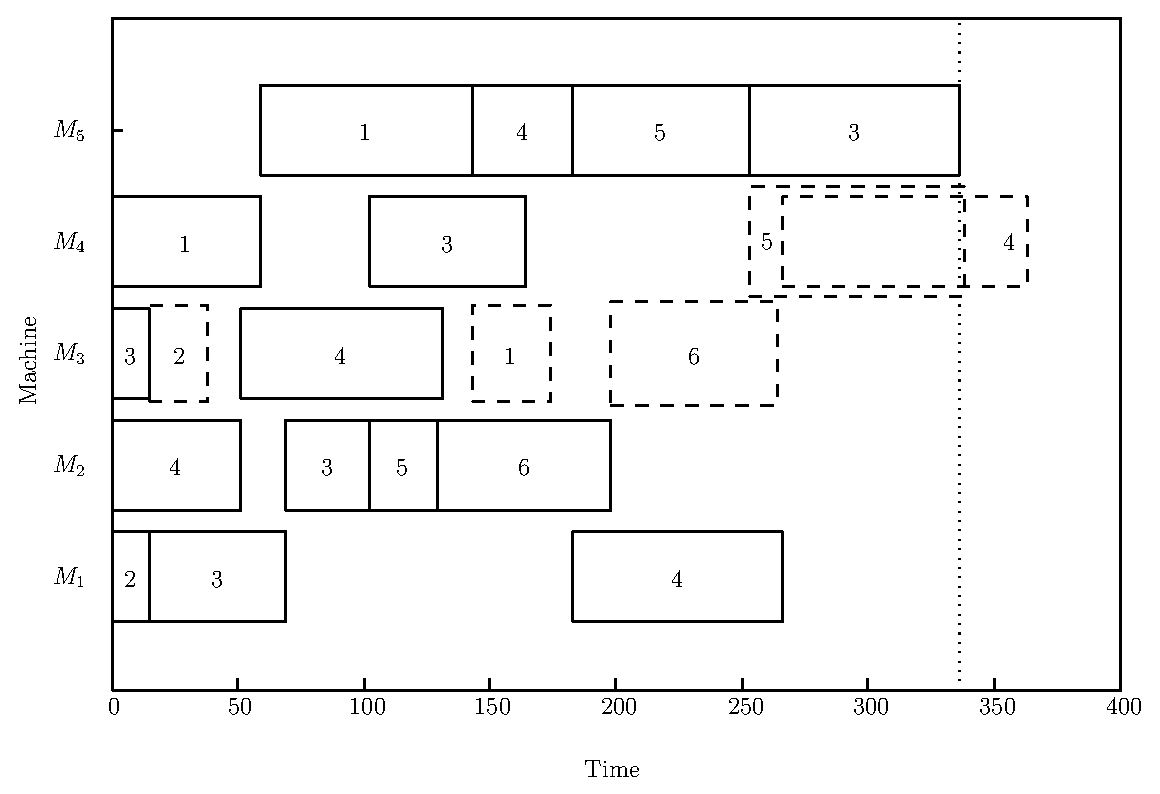
\includegraphics[width=0.8\textwidth]{figures/jssp_example_nocolor.eps}
	\caption[Gantt chart of a partial JSP schedule]{Gantt chart of a
		partial JSP schedule after 15 dispatches: Solid and dashed boxes
		represent $\vchi$ and $\mathcal{L}^{(16)}$, respectively. Current
		$C_{\max}$ denoted as dotted line.}
	\label{fig:jssp:example}
\end{figure}

A \emph{sequence} will refer to the sequential ordering of dispatches of tasks 
to machines, i.e., $(j,a)$; 
the collective set of allocated tasks to machines is interpreted by its 
sequence, is referred to as a \emph{schedule}; 
a \emph{scheduling policy} will pertain to the manner in which 
the sequence is determined.  As shown in our example given in 
\Cref{fig:jssp:example}, there are $15$ operations already scheduled. The 
sequence used to create the schedule was,
\begin{eqnarray}
	\vchi=\left(J_3,J_3,J_3,J_3,J_4,J_4,J_5,J_1,J_1,J_2,J_4,J_6,J_4,J_5,J_3\right)
\end{eqnarray}
and the available jobs to be scheduled
$\mathcal{L}^{(k)}=\{J_1,J_2,J_4,J_5,J_6\}$ describes the five potential jobs 
to be dispatched at step $k=16$ (note that $J_3$ is completed). An overview on 
dispatching rules, used to create such sequences, is given in the following 
\lcnamecref{ch:dispatchrules}.

\subsection{Priority Dispatching Rules}\label{ch:dispatchrules}
% \subsection{Simple priority dispatching rules}
%Dispatching rules are of a construction heuristics, where one starts with an 
%empty schedule and adds sequentially on %one operation (or tasks) at a time. 

A priority dispatching rule inspects the job-list, $\mathcal{L}$, and 
dispatches the job with the highest priority. 
These rules typically use attributes for the corresponding operation, for 
example the processing time for the job. 
Consider again \Cref{fig:jssp:example}, if the job with the shortest processing 
time (SPT) were to be scheduled next then $J_2$ would be dispatched. Similarly, 
for the longest processing time (LPT) heuristic $J_5$ would be dispatched. 
Dispatching can also be based on attributes related to the partial schedule. 
Examples of these are dispatching the job with the most work remaining (MWR) or 
alternatively the least work remaining (LWR). A survey of more than $100$ of 
such rules are presented in \citet{Panwalkar77}, however the reader is referred 
to an in-depth survey for single-priority or \emph{simple dispatching rules} 
(SDR) by \citet{Haupt89}.  SDRs assign an index to each job in the job-list and 
is generally only based on few attributes and simple mathematical operations.

\begin{table}[t!] \centering
	\caption[Attribute space $\mathcal{A}$ for JPS]{Attribute space $\mathcal{A}$ 
		for JSP where job $J_j$ on machine $M_a$ given the resulting temporal 
		schedule after dispatching $(j,a)$.
	}
	\label{tbl:jssp:feat}
	\centering
\renewcommand{\arraystretch}{1.5}
\begin{tabular}{clll} %p{0.45\textwidth}|p{0.4\textwidth}|}
	\toprule
	$\vphi$          & Feature description                       & Mathematical formulation                                                           & Shorthand    \\ 
	%\hline  \multicolumn{4}{c}{\textbf{Local features}}  \\
	\midrule
	\multicolumn{4}{c}{\textbf{job related}}\\
	\phiproc         & job processing time                       & $p_{ja}$                                                                           & proc         \\
	\phistartTime    & job start-time                            & $x_s(j,a)$                                                                         & startTime    \\
	\phiendTime      & job end-time                              & 
	$x_e(j,a)$                                                                    
	     &
	 endTime      \\
	\phiarrivalTime  & job arrival time                          & 
	$x_e(j,a-1)$                                                                  
	     &
	 arrival      \\ 
	\phitotalProc    & total processing time                     & $\sum_{a\in \mathcal{M}}p_{ja}$                                                    & totalProc    \\
	\phiwait         & time job had to wait                      & 
	$x_s(j,a)-x_e(j,a-1) 
	$                                                             & wait         
	\\   
	\phiwrmJob       & total work remaining for job              & $\sum_{a'\in\mathcal{M}\setminus \mathcal{M}_{j}}p_{ja'}$                          & wrmJob       \\
	\phijobOps       & number of assigned operations for job     & $|\mathcal{M}_j|$                                                                  & jobOps       \\ 
	\midrule
	\multicolumn{4}{c}{\textbf{machine related}}\\
	\phimacFree      & when machine is next free                 & $\max_{j'\in 
	\mathcal{J}_a} \{x_e(j',a)\}$                                         & 
	macFree      \\
	\phiwrmMac       & total work remaining for machine          & $\sum_{j'\in\mathcal{J}\setminus \mathcal{J}_{a}}p_{j'a} $                         & wrmMac       \\
	\phimacOps       & number of assigned operations for machine & $|\mathcal{J}_a|$                                                                  & macOps       \\
	\phislotsReduced & change in idle time by assignment         & $\Delta 
	s(a,j)$                                                                    & 
	reducedSlack \\
	\phislots        & total idle time for machine               & $\sum_{j'\in 
	\mathcal{J}_a}s(a,j')$                                                & 
	slack        \\
	\phislotsTotal   & total idle time for all machines          & $\sum_{a'\in 
	\mathcal{M}}\sum_{j'\in \mathcal{J}_{a'}}s(a',j')$                    & 
	totalSlack   \\
	\phimakespan     & current makespan                          & 
	$\max_{(j',a')\in \mathcal{J} \times 
	\mathcal{M}_{j'}}\{x_f(j',a')\}$              & makespan     \\
	\bottomrule
\end{tabular}


\end{table}

Designing priority dispatching rules requires recognizing the important 
attributes of the partial schedules needed to create a good scheduling rule. 
These attributes attempt to grasp key features of the schedule being 
constructed. Which attributes are most important will necessarily depend on the
objectives of the scheduling problem. Attributes used in this study applied for 
a job $J_j$ to be dispatched on machine $M_a$ are given in \cref{tbl:jssp:feat}.
The attributes of particular interest were obtained by inspecting the 
aforementioned SDRs. Attributes \phiJobRelated\ and \phiMacRelated\ are 
job-related and machine-related, respectively. 
Then there are flow-related attributes, \phiFlowRelated\, which measure the 
influence of idle time on the schedule, and current makespan related, 
\phiScheduleRelated.
All of these attributes vary throughout the scheduling process, w.r.t. 
operation belonging to the same time step $k$, with the exception of \phimac, 
which is reported in order to distinguish which features are in conflict with 
each other;
\todo[inline,color=orange!40]{$@$Helga: not sure how this works again... check 
	code, can you recheck if this is all OK here? I mean do we need to talk 
	about things we don't use in our experimental study!
    \\$@$TPR: Features are fine in C\# code. Only discrepancy is with 
    flow-related variable w.r.t. MATLAB code. We use all features from 
    \cref{tbl:jssp:feat} except for \phistep\ and \phiwrmTotal, i.e., total 
    number of features are $d=16$}
\phistep\ to keep track of features' evolution w.r.t. the scheduling process; 
and \phitotalProc\ and \phiwrmTotal\ which are static for a given problem 
instance, but used for normalising other features, e.g., \phiwrmTotal\ for 
work-remaining based ones (\phiwrmJob\ and \phiwrmMac).

Dispatching rules are attractive since they are relatively easy to implement, 
fast and find good schedules. However, they can also fail unpredictably. 
Combining different SDRs can potentially enhance the scheduling performance. 

\subsection{Composite Priority Dispatching Rules}\label{sec:CDR}
A careful combination of dispatching rules can perform significantly better 
\cite{Jayamohan04}. These are referred to as \emph{composite dispatching rules} 
(CDR), where the priority ranking is an expression of several single-based 
priority dispatching rules. CDRs can deal with greater number of features and 
more complicated form, in short, CDR are a combination of several SDRs. For 
instance let CDR be comprised of $d$ dispatching rules (DR), then the index $I$ 
for job $J_j$ using CDR is, 
\begin{equation}
	I_j^{CDR} = \sum_{i=1}^d w_i \cdot \text{DR}_i(\vphi_j) \label{eq:CDR}
\end{equation}
where $w_i>0$ and $\sum_{i=0}^d w_i = 1$ and $w_i$ gives the weight of the 
influence of $\text{DR}_i$ (which could be SDR or another CDR) to CDR. Note, 
each $\text{DR}_i$ is function of the job $J_j$'s attributes $\vphi_j$.  
\nomenclature[zdr2]{CDR}{composite priority dispatching rule}
%\nomenclature[zdr3]{BDR}{blended dispatching rule}

%Since each DR yield a priority index $I^{DR}$ then it is easy to translate its 
%index as a performance measure $a$. Then it is possible to combine several  
%performance measures into a single DR, these are referred to as blended  
%dispatching rules (BDR), where an overall blended priority index $P$ is 
%defined as 
%\begin{equation}
%    P_j = \sum_{a=l} w_a \cdot a 
%\end{equation}
%where $w_a>0$ and $\sum_{a=0}^C w_a = 1$ and $w_a$ gives the weight of the  
%proportional influence of performance measure $a$ (based on some SDR or CDR) 
%to the overall priority.

\todo[inline,color=orange!40]{$@$Helga: can you please make it clear what the 
	difference is between a blended and composite rule, for me its seems to be 
	the same thing... are we confusing things here?!
	\\$@$TPR: You're right, I've commented out the blended dispatching rules. 
	It's hardly ever used in the literature, CDR are much more prevalent name.}

At each time step $k$, an operation is dispatched which has the highest 
priority in the job-list, $\mathcal{L}^{(k)}\subset\mathcal{J}$.  If there is a 
tie, some other priority measure is used. Generally the priority dispatching 
rules are static during the entire scheduling process.

\todo[inline,color=orange!40]{$@$Helga: reword this paragraph so you don't 
	start the sentence with a citation
	\\$@$TPR: I copy/pasted from a document with the NATBIB package, where the 
	\texttt{citet} prints out the author's name, making the sentence human 
	readable.}
Investigating 11 SDRs for JSP, \citet{Lu13} created a pool of 33 composite 
dispatching rules that strongly outperformed the ones they were based on. 
The CDRs were created with multi-contextual functions (MCFs) 
based on either on machine idle time or job waiting time, so one can say that 
the CDRs are a combination of those two key features of the schedule and then 
the SDRs. However, there are no combinations of the basic SDRs explored, only 
machine idle time and job waiting time.  
Similarly, using priority rules to combine 12 existing DRs from the literature, 
\citet{Yu13} had 48 priority rules combinations, yielding 48 different models 
to implement and test. 
It is intuitive to get a boost in performance by introducing new CDRs, since 
where one DR might be failing, another could be excelling so combining them 
together should yield a better CDR. However, these approaches introduce fairly 
ad hoc solutions and there is no guarantee the optimal combination of 
dispatching rules are found.
Moreover, generally the weights $\vec{w}$ are chosen by the designer or the 
rule apriori.  A more attractive approach would be to learn these weights from 
problem examples directly. We will now investigate how this may be accomplished.

\section{Learning Dispatching Rules}\label{ch:learningmodels}
A recent editorial of the state-of-the-art approaches in advanced dispatching 
rules for large-scale manufacturing systems by \citet{Chen13} points out that:
\lq\lq ... most traditional dispatching rules are based on historical data. 
With the emergence of data mining and on-line analytic processing, dispatching 
rules can now take predictive information into account\rq\rq. The importance 
automated discovery of DR was also emphasised by \cite{Monch13}. 
Several of successful implementations in the field of semiconductor wafer 
fabrication facilities are discussed, however, this sort of investigation is 
still in its infancy.

\todo[inline,color=blue!40]{$@$Helga: the remainder of this chapter should be 
	about how learning has been used to find composite dispatching rules, from 
	the literature, here you can cite you own work and the work of Olafson and 
	those citing him. This section should conclude with a paragraph on instance 
	generation and training data creation to connect to the next chapter. I 
	leave this here below in case you would like to use something from it ...}

With meta heuristics one can use existing DRs and use for example 
portfolio-based algorithm selection \citep{Rice76,Gomes01}, either based on a 
single instance or class of instances \citep{Xu07} to determine which DR to 
choose from. 

\citet{Kalyanakrishnan11} point out that meta learning can be very fruitful in 
reinforcement learning, and in their experiments they discovered some key 
discriminants between competing algorithms for their particular problem 
instances, which provided them with a hybrid algorithm which combines the 
strengths of the algorithms.

\citet{Nguyen13} proposed a novel iterative dispatching rules (IDRs) for JSP 
which learns from completed schedules in order to iteratively improve new ones. 
At each dispatching step, the method can utilise the current feature space to 
\emph{correctify} some possible \emph{bad} dispatch made previously (sort of 
reverse lookahead).  Their method is straightforward, and thus easy to 
implement and more importantly computationally inexpensive, although the 
authors do stress that there is still remains room for improvement.

\citet{Korytkowski13} implement ant colony optimisation to select the best DR 
from a selection of nine DRs for JSP and their experiments showed that the 
choice of DR do affect the results and that for all performance measures 
considered it was better to have a all the DRs to choose from rather than just 
a single DR at a time. 	

\section{Learning from Problem Instances}\label{sec:gentrainingdata}
\todo[inline,color=blue!40]{$@$Helga: what is this  chapter is about? This 
chapter need a rewrite, I will let you take the first iteration.}

\subsection{Problem Instances}
\todo[inline,color=orange!40]{$@$Helga: put here all material releated to 
\cref{tbl:data:sim}.\\ 
  $@$TPR: done, was in another section (with subsection field commented)}

For this study synthetic JSP and FSP problem instances will be considered with 
the problem size $10\times10$. 
For each problem space $N_{\text{train}}$  and $N_{\text{test}}$ instances were 
generated for training and testing, respectively. Moreover, of the training 
data 20\% is reserved for validation.
Summary of problem classes is given in \cref{tbl:data:sim}.  
Note, that difficult problem instances are not filtered out beforehand, such as 
the approach in \citet{Whitley}. 


%\subsubsection{Job-shop}\label{data:sim:jssp}
Problem instances for JSP are generated stochastically by fixing the number of 
jobs and machines and discrete processing time are i.i.d. and sampled from a 
discrete uniform distribution from the interval $I=[u_1,u_2]$, i.e., 
$\vec{p}\sim \mathcal{U}(u_1,u_2)$. 
Two different processing times distributions were explored, namely \jrnd{n}{m}  
where $I=[1,99]$ and \jrndn{n}{m}  where $I=[45,55]$.
The machine order is a random permutation of all of the machines in the 
job-shop, hence they problem spaces \jrnd{n}{m}   and \jrndn{n}{m}  are 
referred to as random and random-narrow, respectively. 

Although in the case of \jrnd{n}{m}  this may be an excessively large range for 
the uniform distribution, it is however chosen in accordance with the 
literature \citep{Demirkol98} for creating synthesised $J||C_{\max}$ problem 
instances. In addition, w.r.t. the machine ordering, one could look into a 
subset of JSP where the machines are partitioned into two (or more) sets, where 
all jobs must be processed on the machines from the first set (in some random 
order) before being processed on any machine in the second set, commonly 
denoted as $J|2\textrm{sets}|C_{\max}$ problems, but as discussed in 
\cite{orlib_swv} this family of JSP is considered "hard" (w.r.t. relative error 
from best known solution) in comparison with the "easy" or "unchallenging" 
family with the general $J||C_{\max}$ set-up. % ath. Holtsclaw96 vitnar í 
%orlib_swv um easy-hard pælinguna
This is in stark contrast to \citet{Whitley} whose findings showed that 
structured $F||C_{\max}$ were quite easier to solve than completely random 
structures. 
Intuitively, an inherent structure in machine ordering should be exploitable 
for a better performance.  However, for the sake of generality, a random 
structure is preferred as they correspond to difficult problem instances in the 
case of JSP. 
%Whereas, structured problem subclasses will be explored for FSP.  

%\subsubsection{Flow-shop}\label{data:sim:fsp}
Problem instances for FSP are such that processing times are i.i.d. and 
uniformly distributed, \frnd{n}{m}  where $\vec{p}\sim\mathcal{U}(1,99)$, 
referred to as random. In the JSP context \frnd{n}{m}  is analogous to 
\jrnd{n}{m}. 

\begin{table}\centering
  \caption[Problem space distributions used in experimental studies.]{Problem 
    space distributions used in experimental studies. Note, problem instances 
    are synthetic and each problem space is i.i.d. %and `--' denotes not 
    %available.    
  }\label{tbl:data:sim}
  {\renewcommand{\arraystretch}{1.5}
	\begin{tabular}{clcccl}\toprule 
		type & name & size ($n\times m$) & $N_{\text{train}}$ & 
		$N_{\text{test}}$ & note
		\\ \midrule
		\multirow{2}{*}{{JSP}}
		%&\jrnd{8}{8} &$8\times8$& -- & 500 & random \\
		  & \jrnd{10}{10}  & $10\times10$ & 300 & 200 & random        \\
		%&\jrnd{12}{12} &$12\times12$& -- & 500 & random \\
		%&\jrndn{8}{8} &$8\times8$& -- & 500 & random-narrow \\ 
		  & \jrndn{10}{10} & $10\times10$ & 300 & 200 & random-narrow \\ 
		%&\jrndn{12}{12} &$12\times12$& -- & 500 & random-narrow \\ 
		\midrule
		\multirow{1}{*}{{FSP}}
		%&\frnd{8}{8} &$8\times8$& --&500& random \\ 
		  & \frnd{10}{10}  & $10\times10$ & 300 & 200 & random        \\ 
		%&\frnd{12}{12} &$12\times12$& --&500& random \\ 
		\bottomrule
	\end{tabular}
}
\end{table} 

The goal is to minimize the makespan, $C_{\max}$. The optimum 
makespan is denoted $C_{\max}^{\text{opt}}$, and the makespan obtained from the 
scheduling policy $A$ under inspection by $C_{\max}^{A}$. Since the optimal 
makespan varies between problem instances the performance measure is the 
following,
\begin{equation}\label{eq:ratio}
	\rho=\frac{C_{\max}^{A}-C_{\max}^{\text{opt}}}{C_{\max}^{\text{opt}}}\cdot
	100\%
\end{equation}
which indicates the percentage relative deviation from optimality. %Note, for 
%the OR-Library benchmark suite the optimum is not known, in those instances 
%$C_{\max}^{opt}$ is swapped for $C_{\max}^{BKS}$ which is the latest best 
%known 
%solution reported in the literature. 
\nomenclature[so]{opt}{(known) optimum}
\nomenclature[ss]{sub}{sub-optimum}
\nomenclature[zdr0]{DR}{dispatching rule}
\nomenclature[osizepruned]{$N$}{number of problem instances}

\subsection{Schedule building}\label{sec:gen:gametree}
When building a complete schedule $\ell=n\cdot m$ dispatches must be made 
sequentially.  A job is placed at the earliest available time slot for its next 
machine, whilst still fulfilling that each machine can handle at most one job 
at each time, and jobs need to have finished their previous machines according 
to its machine order. Unfinished jobs are dispatched one at a time according to 
some heuristic. After each dispatch\footnote{Dispatch and time step are used 
	interchangeably.} the schedule's current features (cf. \cref{tbl:jssp:feat}) 
are updated based on the half-finished schedule.

It is easy to see that the sequence of task assignments is by no means unique. 
Inspecting a partial schedule further along in the dispatching process such as 
in \cref{fig:jssp:example}, then let's say $J_1$ would be dispatched next, and 
in the next iteration $J_2$. Now this sequence would yield the same schedule as 
if $J_2$ would have been dispatched first and then $J_1$ in the next iteration, 
i.e., these are non-conflicting jobs.  In this particular instance one can not 
infer that choosing $J_1$ is better and $J_2$ is worse (or vice versa) since
they can both yield the same solution. 

Note that in some cases there can be multiple optimal solutions to the same 
problem instance. Hence not only is the sequence representation `flawed' in the 
sense that slight permutations on the sequence are in fact equivalent w.r.t. 
the end-result, but very varying permutations on the dispatching sequence 
(however given the same partial initial sequence) can result in very different 
complete schedules but can still achieve the same makespan, and thus same 
deviation from optimality, $\rho$, defined by \eqref{eq:ratio}, which is the 
measure under consideration. Care must be taken in this case that neither 
resulting features are labelled as undesirable. Only the resulting features 
from a dispatch resulting in a suboptimal solution should be labelled 
undesirable.

\subsection{Labelling schedules w.r.t. optimal decisions}
The optimum makespan is known for each problem instance. At each time step a 
number of feature pair are created, they consist of the features $\vphi_o$ 
resulting from optimal dispatches $o\in\mathcal{O}^{(k)}$, versus features 
$\vphi_s$ resulting from suboptimal dispatches $s\in\mathcal{S}^{(k)}$ at time 
$k$. Note, $\mathcal{O}^{(k)}\cup\mathcal{S}^{(k)}=\mathcal{L}^{(k)}$ and 
$\mathcal{O}^{(k)}\cap\mathcal{S}^{(k)}=\emptyset$.
In particular, each job is compared against another job of the job-list, 
$\mathcal{L}^{(k)}$, and if the makespan differs, i.e., $C_{\max}^{(s)}\gneq 
C_{\max}^{(o)}$, an optimal/suboptimal pair is created, however if the makespan 
would be unaltered the pair is omitted since they give the same optimal 
makespan. This way, only features from a dispatch resulting in a suboptimal 
solution is labelled undesirable.

The approach taken here is to verify analytically, at each time step, by fixing 
the current temporal schedule as an initial state, whether it can indeed 
\emph{somehow} yield an optimal schedule by manipulating the remainder of the 
sequence. This also takes care of the scenario that having dispatched a job 
resulting in a different temporal makespan would have resulted in the same 
final makespan if another optimal dispatching sequence would have been chosen. 
That is to say the data generation takes into consideration when there are 
multiple optimal solutions to the same problem instance. 

\subsection{Creating time-independent dispatching 
	rules}\label{sec:ord:timeindependent}

Preliminary experiments for creating step-by-step model was done in 
\cite{InRu11a} where an optimal trajectory was explored, i.e., at each dispatch 
some (random) optimal task is dispatched, resulting in local linear model for 
each dispatch; a total of $\ell$ linear models for solving $n\times m$ JSP. 
However, the experiments there showed that by fixing the weights to its mean 
value throughout the dispatching sequence, results remained satisfactory.
A more sophisticated way, would be to create a \emph{new} linear model, where 
the preference set, $S$, is the union of the preference pairs across the $\ell$ 
dispatches. This would amount to a substantial preference set, and for $S$ to 
be 
computationally feasible to learn, $S$ has to be reduced. For this several 
ranking strategies were explored in \cite{InRu15a}, the results there showed 
that it's sufficient to use partial subsequent rankings, namely, combinations 
of $r_i$ and $r_{i+1}$ for $i\in\{1,\ldots,n'\}$, are added to the preference 
set, where $r_1>r_2>\ldots>r_{n'}$ ($n'\leq n$) are the rankings of the 
job-list, $\mathcal{L}^{(k)}$, at time step $k$, in such a manner that in the 
cases that there are more finruthan one operation with the same ranking, only 
one of 
that rank is needed to be compared to the subsequent rank. Moreover, in the 
case of this study, which deals with $10\times 10$ problem instances, the 
partial subsequent ranking becomes necessary, as full ranking is 
computationally infeasible. This is due to the since the size of the preference 
set, $\abs{S}$, becomes too large with full ranking, and would need sampling.
For the following experimental set up, the preference set was limited to 
$\abs{S}\leq200,000$ by random sampling.

\subsection{Linear Learning}
\todo[inline,color=orange!40]{$@$Helga: this is a condensed version of 
    liblinear for our problem, please do not describe logistic regression just 
    how the data is preprocessed and fed into liblinear.
    \\$@$TPR: Duly noted, I've edited that out and simply cited the liblinear 
    package. I also took out the scaling paragraph, as liblinear does that 
    automatically.}

Learning models considered in this study are based on ordinal regression in 
which the learning task is formulated as learning preferences. In the case of 
scheduling, learning which operations are preferred to others. Ordinal 
regression has been previously presented in \cite{Ru06:PPSN} and in 
\cite{InRu11a} for JSP, however given here for completeness. 

Let $\vphi_{o}\in\R^d$ denote the post-decision state when dispatching $J_o$ 
corresponds to an optimal schedule being built. All post-decisions states 
corresponding to suboptimal dispatches, $J_s$, are denoted by 
$\vphi_{s}\in\R^d$. One could label which feature sets were considered optimal, 
$\vec{z}_{o}=\vphi_{o}-\vphi_{s}$, and suboptimal, 
$\vec{z}_{s}=\vphi_{s}-\vphi_{o}$ by $y_o=+1$ and $y_s=-1$ respectively. 
Note, a negative example is only created as long as $J_s$ actually results in a 
worse makespan, i.e., $C_{\max}^{(s)}\gneq C_{\max}^{(o)}$, since there can 
exist situations in which more than one operation can be considered optimal.

The preference learning problem is specified by a set of preference pairs,
\begin{equation}
	S = 
	\left\{\left\{\vec{z}_o,+1\right\}_{k=1}^{\ell},\left\{\vec{z}_s,-1\right\}_{k=1}^{\ell}
	\;|\;\forall o\in \mathcal{O}^{(k)},s\in \mathcal{S}^{(k)}
	\right\}\subset \Phi\times Y \label{eq:Sjssp}
\end{equation}
where $\Phi\subset \mathbb{R}^d$ is the training set of $d$ features,  
$Y=\{-1,+1\}$ is the outcome space, $\ell=n\times m$ is the total number 
dispatches, from which $o\in\mathcal{O}^{(k)}$ and $s\in \mathcal{S}^{(k)}$ 
denote optimal and suboptimal dispatches, respectively, at step $k$. 
Note, $\mathcal{O}^{(k)}\cup\mathcal{S}^{(k)}=\mathcal{L}^{(k)}$, and 
$\mathcal{O}^{(k)}\cap\mathcal{S}^{(k)}=\emptyset$. 

For JSP there are $d=\NrFeatLocal$ features (cf. \cref{tbl:jssp:feat} and 
explained in more detail in \cref{sec:CDR}), and the training set is created in 
the manner described in \cref{sec:gentrainingdata}.
\nomenclature[oe]{$\ell$}{number of dispatches needed for a complete schedule, 
	$\ell=n\cdot m$}
\nomenclature[sk]{$k$}{refers to dispatch/time step $k$ for a schedule}
\nomenclature[ophi]{$\vphi_k$}{feature set, i.e., post-decision state, of a 
(partial) schedule at time $k$}
\nomenclature[od]{$d$}{number of distinct features, i.e., dimension of $\vphi$}
\nomenclature[ophi]{$\Phi$}{training set}
\nomenclature[ophi2]{$S$}{preference set}
\nomenclature[oset1]{$\mathcal{O}^{(k)}$}{set of optimal dispatches at time  
$k$}
\nomenclature[oset2]{$\mathcal{S}^{(k)}$}{set of suboptimal dispatches at time  
$k$}

Now consider the model space $\mathcal{H} = \{h(\cdot) : X \mapsto Y\}$ of 
mappings from solutions to ranks. Each such function $h$ induces an ordering 
$\succ$ on the solutions  by the following rule,
\begin{equation}\label{eq:linear}
	\vec{x}_i \succ \vec{x}_j \quad \Leftrightarrow \quad h(\vec{x}_i) > 
	h(\vec{x}_j)
\end{equation}
where the symbol $\succ$ denotes "is preferred to."  The function used to 
induce the preference is defined by a linear function in the feature space,
\begin{equation}\label{eq:jssp:linweights}
	h(\vec{x})=\sum_{i=1}^d w_i\phi_i(\vec{x})=\inner{\vec{w}}{\vphi(\vec{x})}.
\end{equation}

Logistic regression learns the optimal parameters $\vec{w}^*\in\mathbb{R}^d$. 
For this study, L2-regularized logistic regression from the \textsc{liblinear} 
package \citep{liblinear} without bias is used to learn the preference set $S$, 
defined by \eqref{eq:Sjssp}.
Hence, for each job on the job-list, $J_j\in\mathcal{L}$, let $\vphi_j$ denote 
its corresponding  post-decision state. Then the job chosen to be dispatched, 
$J_{j^*}$, is the one corresponding to the highest preference estimate, i.e.,
\begin{equation}\label{eq:lin}
	J_{j^*}=\argmax_{J_j\in \mathcal{L}}\; h(\vphi_j)
\end{equation}
where $h(\cdot)$ is the classification model obtained by the preference set.

\subsection{Interpreting linear classification 
	models}\label{sec:learningmodels:interpret}
Looking at the features description in \cref{tbl:jssp:feat} it is possible for 
the ordinal regression to `discover' the weights $\vec{w}$ in order for 
\eqref{eq:jssp:linweights} corresponds to applying a single priority 
dispatching rules from \cref{ch:dispatchrules}. For instance, 
\begin{eqnarray*} %{s'rCl}
	SPT:~~w_i&=&\bigg\{ \begin{array}{rl}-1&\text{if 
		}i=1\\0&\text{otherwise}\end{array} \\
	LPT:~~w_i&=&\bigg\{ \begin{array}{rl}+1&\text{if 
		}i=1\\0&\text{otherwise}\end{array} \\
	MWR:~~w_i&=&\bigg\{ \begin{array}{rl}+1&\text{if 
		}i=7\\0&\text{otherwise}\end{array} \\
	LWR:~~w_i&=&\bigg\{ \begin{array}{rl}-1&\text{if 
		}i=7\\0&\text{otherwise}\end{array}
\end{eqnarray*}
where $i\in\{1,\ldots,d\}$. % Note, that at each time step $k$ a task 
%corresponding to the \emph{highest} priority is chosen, i.e., 
%$\argmax_{J_j\in\mathcal{L}}\{h(\vphi_j)\}$.
When using a feature space based on SDRs, the linear classification models can 
very easily be interpreted as CDRs with predetermined weights.



\section{Performance of SDR and BDR}\label{sec:opt}
In order to create successful dispatching rules, a good starting point is to 
investigate the properties of optimal solutions and hopefully be able to learn 
how to mimic such "good" behaviour. For this, we follow an optimal solution, 
obtained by using a commercial software package \cite{gurobi}, and inspect the 
evolution of its features, defined in \cref{tbl:jssp:feat}. Moreover, it is 
noted, that there are several optimal solutions available for each problem 
instance. However, it is deemed sufficient to inspect only one optimal 
trajectory per problem instance as there are $N_{\text{train}}=300$ independent 
instances which gives the training data variety. 

%Note, for this \lcnamecref{sec:opt}, only $10\times10$ problem instances will 
%be considered from the problem spaces described in \cref{tbl:data:sim}. 
%Leaving 
%dimensionality $8\times8$ and $12\times12$ solely for testing scalability in 
%\cref{sec:scalability}. 
%Note, figures within this \lcnamecref{sec:opt} depict the mean over all the 
%training data. %, which are quite noisy functions. Thus, for clarity purposes, 
%%they are fitted with local polynomial regression, making the boundary points 
%%biased.

\subsection{Probability of choosing optimal decision}\label{sec:opt:rnd}
Firstly, we can observe that on a step-by-step basis there are several optimal 
dispatches to choose from. \Cref{fig:opt:unique} depicts how the number of 
optimal dispatches evolve at each dispatch iteration. Note, that only one 
optimal trajectory is pursued (chosen at random), hence this is only a lower 
bound of uniqueness of optimal solutions.
As the number of possible dispatches decrease over time, \cref{fig:opt} depicts 
the probability of choosing an optimal dispatch. 

\begin{figure}
	\centering
	\includegraphics[width=1\linewidth]{figures/{trdat.prob.optUniqueness.10x10.OPT}.pdf}
	\caption{Number of unique optimal dispatches (lower bound)}
	\label{fig:opt:unique}
\end{figure}

\begin{figure}
	\centering
	\includegraphics[width=1\linewidth]{figures/{trdat.prob.moveIsOptimal.10x10.OPT.matlab}.pdf}
	\caption{Probability of choosing optimal move}
	\label{fig:opt}
\end{figure}

\subsection{Making suboptimal decisions}\label{sec:opt:sub}
Looking at \cref{fig:opt}, \jrnd{10}{10}  has a relatively high probability 
($70\%$ and above) of choosing an optimal job. However, it is imperative to 
keep making optimal decisions, because once off the optimal track the 
consequences can be dire. To demonstrate this \cref{fig:case} depicts mean 
worst and best case scenario of the resulting deviation from optimality, 
$\rho$, once you've fallen off the optimal track. Note, that this is given that 
you make \emph{one} wrong turn. Generally, there will be more, and then the 
compound effects of making suboptimal decisions really start adding up. 

It is interesting that for JSP, that over time making suboptimal decisions make 
more of an impact on the resulting makespan. This is most likely due to the 
fact that if suboptimal decision is made in the early stages, then there is 
space to rectify the situation with the subsequent dispatches. However, if done 
at a later point in time, little is to be done as the damage is already 
inflicted upon the schedule. However, for FSP, the case is the exact opposite. 
Then it's imperative to make good decisions right from the beginning. This is 
due to the major structural differences between JSP and FSP, namely the latter 
having a homogeneous machine ordering, constricting the solution immensely. 
Luckily, this does have the added benefit of making it less vulnerable for 
suboptimal decisions later in the decision process. 


\begin{figure}
	\centering
	\includegraphics[width=1\linewidth]{figures/{stepwise.10x10.OPT.casescenario}.pdf}
	\caption{Mean deviation from optimality, $\rho$, (\%), for best (lower 
		bound) and worst (upper bound) case scenario of choosing suboptimal 
		dispatch for \jrnd{10}{10}, \jrndn{10}{10} and \frnd{10}{10}}
	\label{fig:case}
\end{figure}

\subsection{Optimality of simple priority dispatching rules}\label{sec:opt:sdr}
The probability of optimality of the aforementioned SDRs from 
\cref{ch:dispatchrules}, yet still maintaining our optimal trajectory, i.e., 
the probability of a job chosen by a SDR being able to yield an optimal 
makespan on a step-by-step basis, is depicted  in   \cref{fig:opt:SDR}. 
Moreover, the dashed line represents the benchmark of random guessing (cf. 
\cref{fig:opt}).

Now, let's bare in mind the deviation from optimality of applying SDRs 
throughout the dispatching process (box-plots of which are depicted in 
\cref{fig:boxplot:SDR}) then there is a some correspondence between high 
probability of stepwise optimality and low $\rho$. Alas, this isn't always the 
case, for \jrnd{10}{10}, SPT always outperforms LPT w.r.t. stepwise optimality, 
however this does not transcend to SPT having a lower $\rho$ value than LPT. 
Hence, it's not enough to just learn optimal behaviour, one needs to 
investigate what happens once we encounter suboptimal state spaces.

\begin{figure}
	\centering
	\includegraphics[width=1\linewidth]{figures/{trdat.prob.moveIsOptimal.10x10.SDR.matlab}.pdf}
	\caption{Probability of SDR being optimal}
	\label{fig:opt:SDR}
\end{figure}

\begin{figure}
	\centering
	\includegraphics[width=1\linewidth]{figures/{boxplotRho.SDR.10x10}.pdf}
	\caption{Box plot for deviation from optimality, $\rho$, (\%) for SDRs}
	\label{fig:boxplot:SDR}
\end{figure}

\subsection{Simple blended dispatching rule}\label{sec:opt:bdr}
A naive approach to create a simple blended dispatching rule would be for 
instance be switching between two SDRs at a predetermined time point. Hence, 
going back to \cref{fig:opt:SDR} a presumably good BDR for \jrnd{10}{10}  would 
be starting with SPT and then switching over to MWR at around time step 40, 
where the SDRs change places in outperforming one another. A box-plot for 
$\rho$ for all problem spaces is depicted in \cref{fig:boxplot:BDR}. Now, this 
little manipulation between SDRs does outperform SPT immensely, yet doesn't 
manage to gain the performance edge of MWR, save for \frnd{10}{10}. This gives 
us insight that for job-shop based problem spaces, the attribute based on MWR 
is quite fruitful for good dispatches, whereas the same cannot be said about 
SPT -- a more sophisticated BDR is needed to improve upon MWR. 

A reason for this lack of performance of our proposed BDR is perhaps that by 
starting out with SPT in the beginning, it sets up the schedules in such a way 
that it's quite greedy and only takes into consideration jobs with shortest 
immediate processing times. Now, even though it is possible to find optimal 
schedules from this scenario, as \cref{fig:opt:SDR} show, the inherent 
structure that's already taking place, and might make it hard to come across by 
simple methods. Therefore it's by no means guaranteed that by simply swapping 
over to MWR will handle that situation which applying SPT has already created. 
\Cref{fig:boxplot:BDR} does however show, that by applying MWR instead of SPT 
in the latter stages, does help the schedule to be more compact w.r.t. SPT. 
However, in the case of \jrnd{10}{10}  and \jrndn{10}{10}  the fact remains 
that the schedules have diverged too far from what MWR would have been able to 
achieve on its own. Preferably the blended dispatching rule should use  best of 
both worlds, and outperform all of its inherited DRs, otherwise it goes without 
saying one would simply still use the original DR that achieved the best 
results.

\begin{figure}
	\centering
	\includegraphics[width=1\linewidth]{figures/{boxplotRho.BDR.10x10}.pdf}
	\caption{Box plot for deviation from optimality, $\rho$, (\%) for BDR where 
		SPT is applied for the first 40\% of the dispatches, followed by MWR}
	\label{fig:boxplot:BDR}
\end{figure}

\begin{comment}
\subsection{Extremal feature}\label{sec:opt:ext}
The SDRs we've inspected so-far are based on two features from
\cref{tbl:jssp:feat}, namely
\begin{itemize}
	\item \phiproc\ for SPT and LPT 
	\item \phiwrmJob\ for LWR and MWR 
\end{itemize}
by choosing the lowest value for the first SDR, and highest value for the
latter SDR, i.e., the extremal values for those given features. Let's apply the
same methodology from \cref{sec:opt:sdr} to all varying features\footnote{Note,
	\phistep, \phimac\ and \phiwrmTotal\ describe the features, not the schedule.
	For instance, \phistep\, gives us no new information, as that feature is
homogeneous for each time step, making it equivalent to random guessing.} 
described in \cref{tbl:jssp:feat}. 
\Cref{fig:j.rnd:opt:minmax,fig:j.rndn:opt:minmax,fig:f.rnd:opt:minmax} depict
the probability of all extremal features being an optimal dispatch, with random
guessing from \cref{fig:opt} as a dashed line. 

In order to put the extremal features into perspective, it's worth comparing 
them with how the evolution of the features are over time, depicted in 
\cref{fig:j.rnd:opt:evol,fig:j.rndn:opt:evol,fig:f.rnd:opt:evol}. 

\begin{figure}
	\centering
	\includegraphics[width=1\linewidth]{figures/{j.rnd}/{trdat.feat.stepwise.10x10.OPT}.pdf}
	\caption{Feature evolution of optimal trajectory for \jrnd{10}{10}}
	\label{fig:j.rnd:opt:evol}
\end{figure}
\begin{figure}
	\centering
	\missingfigure{j.rndn}
	%\includegraphics[width=1\linewidth]{figures/{j.rndn}/{trdat.feat.stepwise.10x10.OPT}.pdf}
	\caption{Feature evolution of optimal trajectory for \jrndn{10}{10}}
	\label{fig:j.rndn:opt:evol}
\end{figure}
\begin{figure}
	\centering
	\includegraphics[width=1\linewidth]{figures/{f.rnd}/{trdat.feat.stepwise.10x10.OPT}.pdf}
	\caption{Feature evolution of optimal trajectory for \frnd{10}{10}}
	\label{fig:f.rnd:opt:evol}
\end{figure}
\begin{figure}
	\centering
	\includegraphics[width=1\linewidth]{figures/{j.rnd}/{trdat.prob.moveIsOptimal.10x10.feat.minmax}.pdf}
	\caption{Probability of extremal feature being optimal for \jrnd{10}{10}}
	\label{fig:j.rnd:opt:minmax}
\end{figure}
\begin{figure}
	\centering
	\includegraphics[width=1\linewidth]{figures/{j.rndn}/{trdat.prob.moveIsOptimal.10x10.feat.minmax}.pdf}
	\caption{Probability of extremal feature being optimal for \jrndn{10}{10}}
	\label{fig:j.rndn:opt:minmax}
\end{figure}
\begin{figure}
	\centering
	\includegraphics[width=1\linewidth]{figures/{f.rnd}/{trdat.prob.moveIsOptimal.10x10.feat.minmax}.pdf}
	\caption{Probability of extremal feature being optimal for \frnd{10}{10}}
	\label{fig:f.rnd:opt:minmax}
\end{figure}
\end{comment}

\section{Learning CDR}\label{ch:expr:CDR}
\Cref{sec:opt:bdr} demonstrates there is definitely something to be gained by
trying out different combinations, it's just non-trivial how to go about it,
and motivates how it's best to go about learning such interaction, which will
be addressed in this \lcnamecref{ch:expr:CDR}.

\subsection{Feature Selection}
The SDRs we've inspected so-far are based on two features from
\cref{tbl:jssp:feat}, namely
\begin{itemize}
	\item \phiproc\ for SPT and LPT 
	\item \phiwrmJob\ for LWR and MWR 
\end{itemize}
by choosing the lowest value for the first SDR, and highest value for the 
latter SDR, i.e., the extremal values for those given features. 
There is nothing that limits us to using just those two features. 
From \cref{tbl:jssp:feat} we will limit our experiments to the first $d=16$ 
features, as they are varying for each operation, save for \phitotalProc\ which 
is varying for each $J_j\in\mathcal{J}$. 

For this study we will consider all combinations of features using either one,
two, three or all of the features, for a total of
$\nchoosek{d}{1}+\nchoosek{d}{2}+\nchoosek{d}{3}+\nchoosek{d}{d}$, i.e., total
of 697 combinations. The reason for such a limiting number of active features,
are due to the fact we want to keep the models simple enough for improved model
interpretability

For each feature combination, a linear preference model is created in the
manner described in \cref{ch:learningmodels}, where $\Phi$ is limited to the
predetermined feature combination. This was done with the software package from
\cite{liblinear}\footnote{Software available at 
	\url{http://www.csie.ntu.edu.tw/~cjlin/liblinear}},
by training on the full preference set $S$ obtained from the
$N_{\text{train}}=300$ problem instances following the framework set up in
\cref{sec:gentrainingdata}. 
Note, in order to report the validation accuracy, 20\% ($N=60$) of the training 
set was set aside for validation of reporting the accuracy.

\subsection{Validation accuracy}\label{sec:CDR:acc}
As the preference set $S$ has both preference pairs belonging to optimal
ranking, and subsequent rankings, it is not of primary importance to classify
\emph{all} rankings correctly, just the optimal ones. Therefore, instead of
reporting the validation accuracy based on the classification problem of the
correctly labelling the problem set $S$, it's opted the validation accuracy is
obtained in the same manner as done in \cref{sec:opt:sdr} for SDRs, i.e., the
probability of choosing optimal decision given the resulting linear weights,
however in this context, the mean throughout the dispatching process is
reported. \Cref{fig:stepwise_vs_classification} shows the difference between
the two measures of reporting validation accuracy. Validation accuracy based on
stepwise optimality only takes into consideration the likelihood of choosing
the optimal move at each time step. However, the classification accuracy is
also trying to correctly distinguish all subsequent rankings in addition of
choosing the optimal move, as expected that measure is considerably lower. 

\begin{figure}[th!]
	\centering
	\includegraphics[width=\linewidth]{figures/exhaust/{training.accuracy.equal}.pdf}
	\caption{Various methods of reporting validation accuracy for preference 
	learning}
	\label{fig:stepwise_vs_classification}
\end{figure}

\subsection{Pareto front}\label{sec:CDR:pareto}
When training the learning model one wants to keep the validation accuracy 
high, as that would imply a higher likelihood of making optimal decisions, 
which would in turn translate into a low final makespan. To test the validity 
of this assumptions, each of the 697 models is run on the preference set, and 
its mean $\rho$ is reported against its corresponding validation accuracy in 
\cref{fig:CDR:scatter}. The models are colour-coded w.r.t. the number of active 
features, and a line is drawn through its Pareto front. Moreover, those 
solutions are labelled with their corresponding model ID. Moreover, the Pareto 
front over all 697 models, irrespective of active feature count, is denoted 
with triangles. Moreover, their values are reported in \cref{tbl:CDR:pareto}, 
where the best objective is given in boldface. 

For \jrnd{10}{10}  there is no statistical difference between models 2.115, 
3.503, 3.549 and 3.556 w.r.t. $\rho$, however only (2.115, 3.503) and (3.549, 
3.556) w.r.t. validation accuracy. Other models were statistically significant 
to one another, using a Kolmogorov-Smirnov test with 
$\alpha=0.05$.\label{sec:expr:ks} 
However, the solutions on the Pareto front for \jrndn{10}{10} are more or less 
with no (or minimal) statistical difference w.r.t. validation accuracy, and 
considerably fewer w.r.t. $\rho$. Most notably are the 	2.107, 2.115, 3.486 
and 3.549 (latter two have the lowest mean $\rho$) which are all statistically 
insignificant w.r.t. $\rho$ and the latter three w.r.t. validation accuracy as 
well. 
For \frnd{10}{10} 3.80, 3.120, 3.260 are equivalent to model corresponding to 
the lowest $\rho$, 3.244. Although, w.r.t. validation accuracy models 3.260 and 
2.40 are statistically insignificant, where the latter yields a approx 1.5\% 
worse mean $\rho$. So even looking at stepwise optimality by itself is very 
fickle, because slight variations can be quite dramatic to the end result. 

Note, for both \jrnd{10}{10} and \jrndn{10}{10}, model 1.16 is on the Pareto 
front. The model corresponds to feature \phiwrmJob, and in both cases has a 
weight strictly greater than zero (cf. \cref{fig:CDR:weights}). Revisiting 
\cref{sec:learningmodels:interpret}, we observe that this implies the learning 
model was able to discover MWR as one of the Pareto solutions. 

As one can see from \cref{fig:CDR:scatter}, adding additional features to 
express the linear model boosts performance in both validation accuracy and 
expected mean for $\rho$, i.e., the Pareto fronts are cascading towards more 
desirable outcome with higher number  of active features. However, there is a 
cut-off point for such improvement, as using all features is generally 
considerably worse off due to overfitting of classifying the preference set.

\begin{figure}[t]
	\centering
	\includegraphics[width=\linewidth]{figures/exhaust/{pareto.equal}.pdf}
	\caption{Scatter plot for validation accuracy  (\%) against its 
		corresponding mean expected $\rho$ (\%) for all 697 linear models, based on 
		either one, two, three or all $d$ combinations of features.
		Pareto fronts for each active feature count based on maximum validation 
		accuracy and minimum mean expected $\rho$ (\%), and labelled with their 
		model ID. Moreover, actual Pareto front over all models is marked with 
		triangles.} \label{fig:CDR:scatter}
\end{figure}

\begin{table}
	\caption{Mean validation accuracy and mean expected deviation from 
		optimality, $\rho$, for all CDR models on the Pareto front from 
		\cref{fig:CDR:scatter}.}\label{tbl:CDR:pareto}
	\centering
\begin{tabular}{cr@{.}lllc}\toprule
Problem & NrFeat & Model & Acc & $\rho$ & Pareto \\ 
\midrule \multirow{10}{*}{\jrnd} 
   & 1 & 3 & 90.03 & 34.08 &  \\ 
   & 1 & 4 & 74.74 & 21.41 &  \\ 
   & 1 & 16 & 85.43 & 22.06 &  \\ 
   & 2 & 94 & 91.34 & 32.84 &  \\ 
   & 2 & 108 & 91.10 & 13.32 &  \\ 
   & 2 & 115 & 91.08 & 13.31 &  \\ 
   & 3 & 382 & 91.94 & 47.53 &  \\ 
   & 3 & 473 & 91.86 & 23.31 & $\blacktriangle$ \\ 
   & 3 & 549 & 91.68 & \textbf{13.26} & $\blacktriangle$ \\ 
   & 16 & 1 & \textbf{91.95} & 33.96 & $\blacktriangle$ \\ 
\midrule \multirow{11}{*}{\jrndn} 
   & 1 & 4 & 75.38 & 18.84 &  \\ 
   & 1 & 15 & 85.26 & 46.77 &  \\ 
   & 1 & 16 & 84.72 & 19.66 &  \\ 
   & 2 & 113 & 88.53 & 19.66 &  \\ 
   & 2 & 116 & 87.04 & 13.52 &  \\ 
   & 3 & 274 & \textbf{89.82} & 31.39 & $\blacktriangle$ \\ 
   & 3 & 499 & 89.68 & 15.19 & $\blacktriangle$ \\ 
   & 3 & 501 & 87.09 & 13.50 & $\blacktriangle$ \\ 
   & 3 & 508 & 87.07 & \textbf{13.44} & $\blacktriangle$ \\ 
   & 3 & 510 & 87.17 & 14.42 & $\blacktriangle$ \\ 
   & 16 & 1 & 67.48 & 37.66 &  \\ 
\midrule \multirow{7}{*}{\frnd} 
   & 1 & 3 & 81.91 & 18.70 &  \\ 
   & 1 & 8 & 82.55 & 24.45 &  \\ 
   & 2 & 13 & 81.91 & 17.30 &  \\ 
   & 2 & 24 & 85.46 & 17.74 &  \\ 
   & 2 & 51 & 78.72 & 17.17 &  \\ 
   & 3 & 80 & \textbf{85.79} & \textbf{16.72} & $\blacktriangle$ \\ 
   & 16 & 1 & 79.63 & 23.25 &  \\ 
\bottomrule
\end{tabular}

\end{table}

Now, let's inspect the models corresponding to the minimum mean $\rho$ and 
highest mean validation accuracy, highlighted in \cref{tbl:CDR:pareto} and 
inspect the stepwise optimality for those models in \cref{fig:CDR:opt}, again 
using probability of randomly guessing an optimal move from \cref{sec:opt:rnd} 
as a benchmark.
As one can see for both \jrnd{10}{10} and \jrndn{10}{10}, despite having a 
higher mean validation accuracy overall, the probabilities vary significantly. 
A lower mean $\rho$ is obtained when the validation accuracy is gradually 
increasing over time, and especially during the last phase of the 
scheduling.\footnote{It's almost too illegible to notice this shift directly 
	from \cref{fig:CDR:opt}, as the difference between the two best models is 
	oscillating up to only 3\% at any given step. In fact \jrndn{10}{10} has the 
	most clear difference w.r.t. classification accuracy of indicating when a 
	minimum $\rho$ model excels at choosing the preferred move.} Revisiting 
\cref{fig:case}, this trend indicates that it's likelier for the resulting 
makespan to be considerably worse off if suboptimal moves are made at later 
stages, than at earlier stages. Therefore, it's imperative to make the `best' 
decision at the `right' moment, not just look at the overall mean performance. 
Hence, the measure of validation accuracy as discussed in \cref{sec:CDR:acc} 
should take into consideration the impact a suboptimal move yields on a 
step-by-step basis, e.g., weighted w.r.t. a curve such as depicted in 
\cref{fig:case}.

\begin{figure}
	\centering
	\includegraphics[width=0.8\linewidth]{figures/exhaust/{trdat.prob.moveIsOptimal.10x10.OPT.equal.best}.pdf}
	\caption{Probability of choosing optimal move for models corresponding to 
		highest mean validation accuracy (grey) and lowest mean deviation from 
		optimality, $\rho$, (black) compared to the baseline of probability of 
	choosing an optimal move at random (dashed).}
	\label{fig:CDR:opt}
\end{figure}

Let's revert back to the original SDRs discussed in \cref{sec:opt:sdr} and 
compare the best CDR models, a box-plot for $\rho$ is depicted in 
\cref{fig:boxplot:CDR}. Firstly, there is a statistical difference between all 
models, and  clearly the CDR model corresponding to minimum mean $\rho$ value, 
is the clear winner, and outperforms the  SDRs substantially. However, the best 
model w.r.t. maximum validation accuracy, then the CDR model shows a lacklustre 
performance. In some cases it's better off, e.g., compared to LWR, yet for 
job-shop it doesn't surpass the performance of MWR. This implies, the learning 
model is over-fitting the training data. Results hold for the test set. 

\begin{figure}
	\includegraphics[width=1\linewidth]{figures/exhaust/{boxplotRho.CDR.10x10.equal}.pdf}
	\caption{Box plot for deviation from optimality, $\rho$, (\%) for the best 
		CDR models (cf. \cref{tbl:CDR:pareto}) and compared against SDRs from 
		\cref{sec:opt:sdr}, both for training and test sets.}\label{fig:boxplot:CDR}
\end{figure}

\subsection{Interpreting CDR}\label{sec:CDR:interpret}
\Cref{sec:learningmodels:interpret} showed how to interpret the linear 
preference models by their weights. 
\Cref{fig:CDR:weights} depicts the linear weights, $\vec{w}$, from 
\cref{eq:linear} for all of the CDR models reported in \cref{tbl:CDR:pareto}. 
The weights have been normalised for clarity purposes, such that it is scaled 
to $\norm{\vec{w}}=1$, thereby giving each feature their proportional 
contribution to the  preference $I_j^{CDR}$ defined by \cref{eq:CDR}.

%Part of 10x10.joh.Features run, now no longer apart of the Pareto-front so not 
%in the main table
%As discussed in \cref{sec:expr:ks} for \jrndn{10}{10}, there is no statistical 
%difference between models 3.501, 3.508 and 3.510 w.r.t. validation accuracy. 
%As 
%\cref{fig:CDR:weights} shows, \phimakespan\ and \phiwrmJob\  are similar in 
%value, however it's the third feature that yields the difference in 
%performance. In fact, the contribution from \phiproc\ in 3.501 is on par with 
%\phimac\ in 3.508, as those models are not statistically different w.r.t. 
%$\rho$ performance. However, the decreased contribution of \phimakespan\  in 
%favour for \phimacFree\ in 3.510 results in approximately 1\% increase in 
%$\rho$. Furthermore, it's sufficient to use only \phimakespan\ and 
%\phiwrmJob\  
%as active features, as model 2.116 has no statistical difference from either 
%3.508 or 3.510, for both $\rho$ and validation accuracy.

For \jrndn{10}{10}, there is no statistical difference between models 2.116 and 
3.521 w.r.t. either $\rho$ or validation accuracy. As \cref{fig:CDR:weights} 
shows, \phimakespan\ and \phiwrmJob\  are similar in value. However, looking at 
model 3.502 which has a slight statistical difference w.r.t. accuracy, the 
third feature yields the staggering difference in performance, about 20\% 
increase in $\rho$. 
It's also interesting to inspect the full model for \frnd{10}{10}, 16.1. 
Despite having similar contributions as all the active features of one of the 
its best model, 3.80, then the substantial interference from \phijobOps\ along 
with other features present, hinders the full model from achieving a low 
$\rho$, thereby stressing the importance of feature selection, to steer clear 
of over-fitting. 

Furthermore, in the case of  models 3.80 and 3.120 for \frnd{10}{10} 
(equivalent both w.r.t. $\rho$ and accuracy) the only difference is features 
\phiendTime\ and \phimacFree. 
In addition, models 3.549 and 3.556 for \jrnd{10}{10} show the same behaviour. 
As these features often coincide in job-shop, it is justifiable to use only 
either one, as the it contains the same information as its counterpart. 
Assuming this holds, then for models 3.498 and 3.503 where there is similar 
contributions between \phimacFree\ and \phiendTime, respectively, and 
\phiwrmJob\ for both, the weights are similar, yet statistically significant 
from one another. There the third feature is the key to the success of the CDR, 
as opting for \phimakespan\ instead of \phiwait\ for 3.503 boosts the $\rho$ 
performance by 8.6\%. 
In addition, models 2.115 and 3.498, have similar contributions for 
\phimacFree\ and \phiwrmJob, however the additional \phiwait, which causes the 
performance of $\rho$ to diminish by 8.5\%.

\begin{figure}
	\centering
	\includegraphics[width=\textwidth]{figures/exhaust/{pareto.equal.phi.j.rnd}.pdf}\\
	\includegraphics[width=\textwidth]{figures/exhaust/{pareto.equal.phi.j.rndn}.pdf}\\
	\includegraphics[width=\textwidth]{figures/exhaust/{pareto.equal.phi.f.rnd}.pdf}
	\caption{Normalised weights for CDR models from \cref{tbl:CDR:pareto}, 
		models are grouped w.r.t. its dimensionality, $d$. Note, a triangle 
		indicates a solution on the Pareto front.}\label{fig:CDR:weights}
\end{figure}

\section{Conclusions}\label{sec:con}
Current literature still hold single priority dispatching rules in high regard, 
as they are simple to implement and quite efficient. 
However, they are generally taken for granted as there is clear lack of 
investigation of \emph{how} these dispatching rules actually work, and what 
makes them so successful (or in some cases unsuccessful)? 
For instance, of the four SDRs this study focuses on, why does MWR outperform 
so significantly for job-shop, yet completely fail for flow-shop? 
MWR seems to be able to adapt to varying distributions of processing times, 
however manipulating the machine ordering causes MWR to break down. 
By inspecting optimal schedules, and meticulously researching what's going on, 
every step of the way of the dispatching sequence, some light is shed where 
these SDRs vary w.r.t. the problem space at hand. \todo{"What general lessons 
might be learnt from this study?"}
Once these simple rules are understood, then it's feasible to extrapolate the 
knowledge gained and create new composite rules that are likely to be 
successful. 

Creating new dispatching rules is by no means trivial. For job-shop there is 
the hidden interaction between processing times and machine ordering that's 
hard to measure.
Due to this artefact, feature selection is of paramount importance, and then it 
becomes the case of not having too many features, as they are likely to hinder 
generalisation due to over-fitting in training. However, the features need to 
be explanatory enough to maintain predictive ability. 
For this reason \cref{ch:expr:CDR} was limited to up to three active features, 
as the full feature set was clearly sub-optimal w.r.t. the SDRs used as a 
benchmark. 
By using features based on the SDRs, along with some additional local features 
describing the current schedule, it was possible to `discover' the SDRs when 
given only one active feature. %Although there is not much to be gained by 
%these models, they at least are a sanity check the learning models are on the 
%right track. 
Furthermore, by adding on additional features, a boost in performance was 
gained, resulting in a composite dispatching rule that outperformed all of the 
SDR baseline. 

When training the learning model, it's not sufficient to only optimize w.r.t. 
highest mean validation accuracy. As \cref{sec:CDR:pareto} showed, there is a 
trade-off between making the over-all best decisions versus making the right 
decision on crucial time points in the scheduling process, as \cref{fig:case} 
clearly illustrated. It is for this reason, traditional feature selection such 
as add1 and drop1 were unsuccessful in preliminary experiments, and thus 
resorting to having to exhaustively search all feature combinations.
This also opens of the question of how should validation accuracy be measured? 
Since the model is based on learning preferences, both based on optimal versus 
suboptimal, and then varying degrees of sub-optimality. As we are only looking 
at the ranks in a black and white fashion, such that the makespans need to be 
strictly greater to belong to a higher rank, then it can be argued that some 
ranks should be grouped together if their makespans are sufficiently close. 
This would simplify the training set, making it (presumably) less of 
contradictions and more appropriate for linear learning. Or simply the 
validation accuracy could be weighted w.r.t. the  difference in 
makespan.\todo{Future work topic \#1}

During the dispatching process, there are some pivotal times which need to be 
especially taken care off. \Cref{fig:case} showed how making suboptimal 
decisions were more of a factor during the later stages, whereas for flow-shop 
the case was exact opposite. \todo{Going to wait with this section until 
	\cref{sec:sampling} has been completed}

Despite the abundance of information gathered by following an optimal 
trajectory, the knowledge obtained is not enough by itself. Since the learning 
model isn't perfect, it is bound to make a mistake eventually. When it does, 
the model is in uncharted  territory as there is not certainty the samples 
already collected are able to explain the current situation. For this we 
propose investigating features from suboptimal trajectories as well, since the 
future observations depend on previous predictions. 
\todo{Future work topic \#2} A straight forward approach would be to inspect 
the trajectories of promising SDRs or CDRs. 
In fact, it would be worth while to try out imitation learning by 
\cite{RossB10,RossGB11}, such that the learned policy following an optimal 
trajectory is used to collect training data, and the learned model is updated. 
This can be done over several iterations, with the benefit being, that the 
states that are likely to occur in practice are investigated, and as such used 
to dissuade the model from making poor choices. Alas, this comes at great 
computational cost due to the substantial amounts of states that need to be 
optimised for their correct labelling. Making it only practical for job-shop of 
a considerable lower dimension. \todo{Future work topic \#3}

Although this study has been structured around the job-shop scheduling problem, 
it is easily extended to other types of deterministic optimisation problems 
that involve sequential decision making. \todo{Place work in wider context}	
The framework presented here collects snap-shots of the state space by 
following an optimal trajectory, and verifying the resulting optimal makespan 
from each possible state. 
From which the stepwise optimality of individual features can be inspected, 
which could for instance justify omittance in feature selection. \todo{Not 
done, but possible} 
Moreover, by looking at the best and worst case scenario of suboptimal 
dispatches, it is possible to pinpoint vulnerable times in the scheduling 
process. 

\bibliographystyle{spmpsci} % spmpsci ??
\bibliography{../references}  

%\clearpage \listoftodos[Todo and remarks]
\end{document}

\section{Scheduling Heuristics} \label{sec:constructionjssp}
Heuristics algorithms for scheduling are typically either a construction or 
improvement heuristics. The improvement heuristic starts with a complete 
schedule and then tries to find similar, but better schedules.  A construction 
heuristic starts with an empty schedule and adds one job at a time until the 
schedule is complete.
The work presented here will focus on construction heuristics, although the 
techniques developed could be adapted to improvement heuristics also.  In 
scheduling a construction heuristic is typically implemented as a priority 
dispatching rule.  These are simple rules that basically determine which 
uncompleted job should be dispatched next.  However, knowing which job to 
dispatch is not sufficient, one must also know where to place it.  In order to 
build tight schedules it would be sensible to place the jobs, once they become 
available, such that the machine idle time is minimal. There may also be a 
number of different options for such a placement.
\Cref{fig:jssp:example} illustrates the dispatching process with an example of 
a temporal partial schedule for six jobs scheduled on five-machines.  The 
numbers in the boxes represent the job's identification $j$.  The width of the 
box illustrates the processing times for a given job for a particular machine 
$M_a$ (on the vertical axis).  The dashed boxes represent the resulting partial 
schedule for when a particular job is scheduled next.  Moreover, the current
$C_{\max}$ is denoted with a dotted horizontal line.  In the figure one observes
that $J_2$, to be scheduled on $M_3$, could be placed immediately in a slot 
between $J_3$ and $J_4$, or after $J_4$.  If $J_6$ had been scheduled prior a 
slot would have been created between it and $J_4$, thus creating a third 
alternative where $J_2$ is placed after $J_6$.  The construction heuristic must 
therefore decide where to place the job, and this may be independent of the 
dispatching rule applied.  Different placement strategies could be considered, 
for example placing a job in smallest feasible slot.  In our preliminary
experiments we have discovered that such a placement could rule out the 
possibility of constructing solutions with an optimal makespan. This problem 
did not occur when jobs were simply placed as early as feasibly possible.

\begin{figure}[t!]\centering
	\includegraphics[width=0.8\textwidth]{figures/jssp_example_nocolor-eps-converted-to.pdf}
	\caption[Gantt chart of a partial JSP schedule]{Gantt chart of a
		partial JSP schedule after 15 dispatches: Solid and dashed boxes
		represent $\vchi$ and $\mathcal{L}^{(16)}$, respectively. Current
		$C_{\max}$ denoted as dotted line.}
	\label{fig:jssp:example}
\end{figure}

A \emph{sequence} will refer to the sequential ordering of the dispatches of 
tasks to machines, i.e., $(j,a)$; the collective set of allocated tasks to 
machines, which is interpreted by its sequence, is referred to as a 
\emph{schedule}; a \emph{scheduling policy} will pertain to the manner in which 
the sequence is determined.  As shown in our example given in 
\Cref{fig:jssp:example}, there are 15 operations already scheduled. The 
sequence used to create the schedule was,
\begin{eqnarray}
	\vchi=\left(J_3,J_3,J_3,J_3,J_4,J_4,J_5,J_1,J_1,J_2,J_4,J_6,J_4,J_5,J_3\right)
\end{eqnarray}
hence the current available jobs to be scheduled 
$\mathcal{L}=\{J_1,J_2,J_4,J_5,J_6\}$, and will be referred to as our job-list, 
describes the 5 potential jobs to be dispatched at step $k=16$ (note that $J_3$ 
is completed).
